% SAPHIR — AAMAS 2027 Blue Sky Ideas track draft (v0.1)
% Compile: pdflatex main.tex
\documentclass[10pt,twocolumn]{article}
\usepackage[margin=0.7in]{geometry}
% (default Computer Modern; add mathptmx/lmodern on full TeX installs)
\usepackage{booktabs}
\usepackage{graphicx}
\usepackage{hyperref}
\usepackage{tikz}
\usetikzlibrary{arrows.meta,positioning}
\setlength{\columnsep}{0.25in}
\title{SAPHIR: Secure Acoustic Pairing for Heterogeneous Inter-agent Rendezvous\\{\normalsize Beyond Speech for Agent-to-Agent Dialogue on Bare Audio Channels}}
\author{Rathod Vaibhav Vishwas Ram\\{\small Department of Computer Science and Engineering, R.~V.~College of Engineering, Bengaluru, India}\\\small\texttt{github.com/vaibhav-rm/SAPHIR}}
\date{\small Draft v0.1 --- October 2026 (AAMAS 2027 Blue Sky Ideas)}
\begin{document}
\maketitle

\begin{abstract}
Voice AI agents that call each other still converse the wasteful way:
speech~$\to$~text~$\to$~LLM~$\to$~speech, even when both sides are machines.
The viral Gibberlink demo (Feb.\ 2025) showed two agents can instead switch to
data-over-sound tones --- but with no authentication, no negotiation, no
structure, and no audit trail: anyone with a speaker can spoof it.
Meanwhile the emerging interop stack (MCP, A2A, ANP, InterSAGE) uniformly
assumes IP connectivity and HTTPS, leaving voice-only calls, PSTN trunks,
offline rooms, and noisy acoustic channels uncovered.
We argue the community needs \emph{acoustic pairing}: any two heterogeneous
agents sharing nothing but a bare audio channel should detect each other,
negotiate a codec, establish forward-secret encryption, and collaborate in
structured tasks --- while every beep stays human-inspectable.
We sketch SAPHIR, a three-phase handshake (HELLO~$\to$~WELCOME~$\to$~KEY1~$\to$~KEY2)
followed by AEAD-encrypted CBOR tasks, and report preliminary evidence from an
open prototype: sub-150\,B task frames, blocked spoof/replay/downgrade attacks,
and a quantified robustness cliff that motivates reliability framing as the next
step. We close with three research questions for the community.
\end{abstract}

\section{Introduction}
In February 2025 two engineers demonstrated Gibberlink~\cite{gibberlink}: two
voice agents on a phone call realize both sides are AI and switch from English
to \texttt{ggwave}~\cite{ggwave} data-over-sound tones --- bleeps that carry
text faster than speech and skip two speech-synthesis passes. The video passed
15M views. The technical content, however, is a prompt (``switch if the other
side is AI'') plus raw tones: the switch is \emph{unauthenticated}, the format
is \emph{unnegotiated}, the content is still \emph{unstructured English}, and
the exchange is \emph{opaque to humans}. A recorded beep replays; a crafted
beep injects; a legacy peer is silently beeped at.

The same year, the agent-interop community converged on a serious stack for
agent collaboration: MCP for agent-to-tool access, A2A for task delegation with
Agent Cards, ANP for decentralized discovery, and InterSAGE for the
identity/trust substrate~\cite{interop-survey,intersage}. Its threat models are
maturing just as fast: A2ASecBench~\cite{a2asecbench} and ASB show protocol-logic
attacks bypassing default safeguards, and Dangol~\cite{graphmeta} shows even
encrypted transports leak the communication graph. Yet every one of these
protocols assumes URL-addressable agents over HTTP(S). None answers: \emph{what
if the only shared channel is sound?}

That gap is not exotic. Near-term agent telephony (AI receptionists, AI
assistants calling businesses), PSTN trunks that mangle ultrasound, hospitals
and plants where RF is restricted, and disaster/offline settings all produce
voice-only encounters between heterogeneous agents. This paper's thesis:
\emph{agent pairing over bare audio deserves first-class protocol status, with
security and auditability designed in --- not demoed around.}

\section{Vision: pairing like Bluetooth}
We envision \emph{acoustic pairing}: two agents that share nothing but a
microphone and a speaker should, within seconds:
\begin{enumerate}
\item \textbf{Detect} mutual AI capability without trusting self-declaration alone;
\item \textbf{Negotiate} codecs and task ontologies in tens of bytes;
\item \textbf{Encrypt} with per-pairing forward secrecy, cheap enough for tones;
\item \textbf{Collaborate} in structured intents (slots, not sentences);
\item \textbf{Account} for every exchange in a human-readable sidecar log.
\end{enumerate}
Properties 1--4 deliver Gibberlink's promised efficiency; property 5 answers
the trust gap Cisco reports as the top blocker of agentic-AI deployment (85\%
exploring, 5\% in production~\cite{ciscotrust}): beeps the operator cannot read
are a non-starter for high-stakes tasks.

\section{Why the HTTP stack does not solve it}
Table~\ref{tab:stack} positions acoustic pairing against the 2025--26 stack.
The pattern is uniform: content standardized, transport assumed. IETF drafts on
agent-protocol frameworks~\cite{ietf-agents} explicitly list discovery,
negotiation, and fallback among open requirements --- precisely the pieces a
bare-audio channel forces us to re-derive under a $\sim$30\,Bps budget with no
PKI handshake room and codecs that destroy ultrasound.

\begin{table}[h]
\centering\small
\caption{Acoustic pairing vs.\ the interop stack. All prior rows assume IP.}
\label{tab:stack}
\begin{tabular}{@{}llll@{}}
\toprule
System & Channel & Auth & Audio fallback \\
\midrule
Gibberlink & audio only & none (prompt) & itself, insecure \\
MCP & HTTPS tool & yes & none \\
A2A & HTTPS agent & yes & none \\
ANP & HTTPS + DID & yes & none \\
InterSAGE & trust substrate & yes & none \\
\textbf{SAPHIR (this work)} & \textbf{audio / hybrid} & \textbf{eph.\ keys} & \textbf{native} \\
\bottomrule
\end{tabular}
\end{table}

\section{SAPHIR sketch}
SAPHIR (Secure Acoustic Pairing for Heterogeneous Inter-agent Rendezvous) is a
minimal pairing protocol; our prototype implements it in $\sim$800 lines of
Python (\url{github.com/vaibhav-rm/SAPHIR}).
Frames are length-prefixed CBOR envelopes,
\texttt{u32be len $\parallel$ CBOR(\{v,type,seq,sender,nonce,payload\})}, capped
at 200\,B. The handshake (Fig.~\ref{fig:hs}) is: \textbf{HELLO} (ephemeral
\texttt{did:key}, codec list), \textbf{WELCOME} (selected codec --- a peer
offering no SAPHIR codec is flagged and kept in English, never silently
beeped at), \textbf{KEY1/KEY2} (32\,B X25519 ephemeral keys each way
$\to$ HKDF-SHA256 $\to$ 32\,B ChaCha20-Poly1305 session key), then
\textbf{TASK/RESULT} pairs as \texttt{ChaCha(cbor(\{intent,slots,ontology,ts\}))}
with the sender bound as AAD and replays rejected by sequence plus (nonce, ct)
sets. Deliberately out of scope for v0.1: PKI-backed identity, MLS groups,
ultrasound modes, and retransmission.

\begin{figure}[h]
\centering
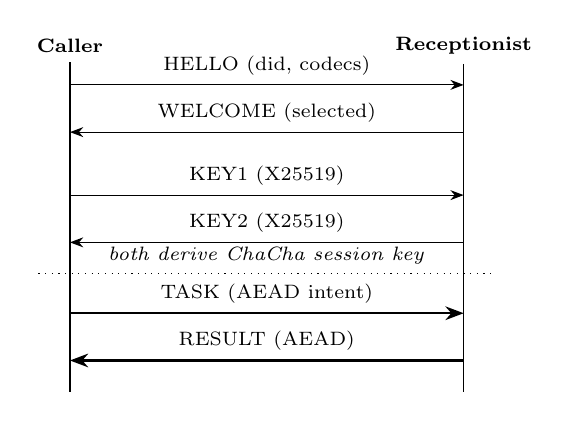
\begin{tikzpicture}[font=\scriptsize, >=Stealth]
\node (A) at (0,0) {\textbf{Caller}};
\node (B) at (5,0) {\textbf{Receptionist}};
\draw (A) -- (0,-4.4); \draw (B) -- (5,-4.4);
\draw[->] (0,-0.5) -- (5,-0.5) node[midway,above] {HELLO (did, codecs)};
\draw[->] (5,-1.1) -- (0,-1.1) node[midway,above] {WELCOME (selected)};
\draw[->] (0,-1.9) -- (5,-1.9) node[midway,above] {KEY1 (X25519)};
\draw[->] (5,-2.5) -- (0,-2.5) node[midway,above] {KEY2 (X25519)};
\draw[dotted] (-0.4,-2.9) -- (5.4,-2.9) node[above,midway] {\textit{both derive ChaCha session key}};
\draw[->,thick] (0,-3.4) -- (5,-3.4) node[midway,above] {TASK (AEAD intent)};
\draw[->,thick] (5,-4.0) -- (0,-4.0) node[midway,above] {RESULT (AEAD)};
\end{tikzpicture}
\caption{SAPHIR pairing: plaintext negotiation, then encrypted tasks. Every frame is sidecar-logged with its decrypted view.}
\label{fig:hs}
\end{figure}

The threat model is summarized in Table~\ref{tab:threat}: the three attacks that
succeed trivially against raw-tone switching are blocked by construction, while
stolen-session keys and traffic analysis are declared out of scope (cf.\
InterSAGE~\cite{intersage} and~\cite{graphmeta} for the IP-side treatment).

\begin{table}[h]
\centering\small
\caption{Threat model: raw tones vs.\ SAPHIR v0.1 (prototype-verified).}
\label{tab:threat}
\begin{tabular}{@{}lll@{}}
\toprule
Attack & Raw tones & SAPHIR \\
\midrule
Tone spoof / injection & succeeds & blocked (AEAD tag) \\
Replay of valid frame & succeeds & blocked (seq + nonce set) \\
Forced downgrade & silent & flagged, stays in English \\
Eavesdropping & plaintext & ciphertext \\
Stolen session keys & n/a & out of scope (needs PKI) \\
Who-talks-to-whom & n/a & out of scope \\
\bottomrule
\end{tabular}
\end{table}

\section{Preliminary evidence}
Our prototype runs the full pairing plus a hotel-booking task (check then book)
with no audio hardware (byte-identical framing; over-air as next step).
Measured envelope sizes: HELLO $\sim$194\,B, KEY $\sim$107--113\,B,
TASK \texttt{hotel.check} 117\,B and \texttt{hotel.book} 131\,B with dictionary
coding (\texttt{date}$\to$\texttt{d}, \texttt{hotel.book}$\to$\texttt{hb}, value
shorts, omitted default ontology; legacy full-form still decodes). A scripted attacker without session keys is
rejected (\texttt{InvalidTag}); an exact replay is rejected (sequence reuse);
a legacy peer is kept in English with an explicit flag ---
all three checks run as \texttt{evals/attacks.py}.
A 50-trial/cell loss sweep (\texttt{evals/robustness.py}) shows 100\% success
on a clean channel, 94\% at 1\% frame loss degrading to 44\% at 10\% loss, and
a sharp corruption cliff (36\% at 0.1\% byte-corruption, 0\% at 0.5\%) ---
expected, since AEAD must reject forgeries, and precisely the quantification
that motivates ACK/retry framing next. Two genuine bugs (a shallow-copied
inventory, a RESULT decoder mangling) were caught by the sweep itself.

\section{Open challenges}
We propose three questions for the community.
\textbf{(RQ1)} What is the minimal negotiable handshake under $\sim$30\,Bps
with codecs that destroy ultrasound --- can Agent-Card semantics compress into
tens of bytes? \textbf{(RQ2)} How should semantic (not textual) agreement be
verified over such channels, given that well-formed JSON does not imply shared
meaning~\cite{semalign}? \textbf{(RQ3)} What does auditability mean when the
channel is human-inaudible --- selective disclosure of the sidecar without
leaking the workflow graph~\cite{graphmeta}? Our roadmap (reliability framing,
sub-140\,B compaction, ephemeral-DID PKI, over-air measurements across
PCM/Opus/G.711) is documented with the artifact; we invite red-teamers.

\begin{thebibliography}{9}
\bibitem{gibberlink} B.~Starkov and A.~Pidkuiko. GibberLink, 2025. \texttt{github.com/PennyroyalTea/gibberlink}.
\bibitem{ggwave} G.~Gerganov. ggwave: data-over-sound library. \texttt{github.com/ggerganov/ggwave}.
\bibitem{interop-survey} A.~Ehtesham et al. A survey of agent interoperability protocols: MCP, ACP, A2A, and ANP. arXiv:2505.02279, 2025.
\bibitem{intersage} Z.~Zou et al. InterSAGE: the secure and verifiable interoperability protocol for an internet of agents. arXiv:2608.13030, 2026.
\bibitem{a2asecbench} T.~Li et al. A2ASecBench: a protocol-aware security benchmark for agent-to-agent multi-agent systems. ICLR, 2026.
\bibitem{graphmeta} B.~Dangol. From privacy to workflow integrity: communication-graph metadata in autonomous agent interoperability. arXiv:2606.07150, 2026.
\bibitem{semalign} Beyond message passing: toward semantically aligned agent communication. arXiv:2604.02369.
\bibitem{ietf-agents} J.~Rosenberg. Framework, use cases and requirements for AI agent protocols. IETF draft-rosenberg-ai-protocols, 2025; Y.~Cui. Cross-domain interoperability framework. draft-cui-dmsc-agent-cdi, 2026.
\bibitem{ciscotrust} Cisco. The agent trust gap: what our research reveals about agentic AI security. 2026.
\end{thebibliography}
\end{document}
